% Template for PLoS
% Version 3.5 March 2018
%
% % % % % % % % % % % % % % % % % % % % % %
%
% -- IMPORTANT NOTE
%
% This template contains comments intended 
% to minimize problems and delays during our production https://www.overleaf.com/project/5e7a9efde3becb000141fd9b
% process. Please follow the template instructions
% whenever possible.
%
% % % % % % % % % % % % % % % % % % % % % % % 
%
% Once your paper is accepted for publication, 
% PLEASE REMOVE ALL TRACKED CHANGES in this file 
% and leave only the final text of your manuscript. 
% PLOS recommends the use of latexdiff to track changes during review, as this will help to maintain a clean tex file.
% Visit https://www.ctan.org/pkg/latexdiff?lang=en for info or contact us at latex@plos.org.
%
%
% There are no restrictions on package use within the LaTeX files except that 
% no packages listed in the template may be deleted.
%
% Please do not include colors or graphics in the text.
%
% The manuscript LaTeX source should be contained within a single file (do not use \input, \externaldocument, or similar commands).
%
% % % % % % % % % % % % % % % % % % % % % % %
%
% -- FIGURES AND TABLES
%
% Please include tables/figure captions directly after the paragraph where they are first cited in the text.
%
% DO NOT INCLUDE GRAPHICS IN YOUR MANUSCRIPT
% - Figures should be uploaded separately from your manuscript file. 
% - Figures generated using LaTeX should be extracted and removed from the PDF before submission. 
% - Figures containing multiple panels/subfigures must be combined into one image file before submission.
% For figure citations, please use "Fig" instead of "Figure".
% See http://journals.plos.org/plosone/s/figures for PLOS figure guidelines.
%
% Tables should be cell-based and may not contain:
% - spacing/line breaks within cells to alter layout or alignment
% - do not nest tabular environments (no tabular environments within tabular environments)
% - no graphics or colored text (cell background color/shading OK)
% See http://journals.plos.org/plosone/s/tables for table guidelines.
%
% For tables that exceed the width of the text column, use the adjustwidth environment as illustrated in the example table in text below.
%
% % % % % % % % % % % % % % % % % % % % % % % %
%
% -- EQUATIONS, MATH SYMBOLS, SUBSCRIPTS, AND SUPERSCRIPTS
%
% IMPORTANT
% Below are a few tips to help format your equations and other special characters according to our specifications. For more tips to help reduce the possibility of formatting errors during conversion, please see our LaTeX guidelines at http://journals.plos.org/plosone/s/latex
%
% For inline equations, please be sure to include all portions of an equation in the math environment.  For example, x$^2$ is incorrect; this should be formatted as $x^2$ (or $\mathrm{x}^2$ if the romanized font is desired).
%
% Do not include text that is not math in the math environment. For example, CO2 should be written as CO\textsubscript{2} instead of CO$_2$.
%
% Please add line breaks to long display equations when possible in order to fit size of the column. 
%
% For inline equations, please do not include punctuation (commas, etc) within the math environment unless this is part of the equation.
%
% When adding superscript or subscripts outside of brackets/braces, please group using {}.  For example, change "[U(D,E,\gamma)]^2" to "{[U(D,E,\gamma)]}^2". 
%
% Do not use \cal for caligraphic font.  Instead, use \mathcal{}
%
% % % % % % % % % % % % % % % % % % % % % % % % 
%
% Please contact latex@plos.org with any questions.
%
% % % % % % % % % % % % % % % % % % % % % % % %

\documentclass[10pt,letterpaper]{article}
\usepackage[top=0.85in,left=2.75in,footskip=0.75in]{geometry}

% amsmath and amssymb packages, useful for mathematical formulas and symbols
\usepackage{amsmath,amssymb}

% Use adjustwidth environment to exceed column width (see example table in text)
\usepackage{changepage}

% Use Unicode characters when possible
\usepackage[utf8x]{inputenc}

% textcomp package and marvosym package for additional characters
\usepackage{textcomp,marvosym}

% cite package, to clean up citations in the main text. Do not remove.
\usepackage{cite}

% Use nameref to cite supporting information files (see Supporting Information section for more info)
\usepackage{nameref,hyperref}

% line numbers
\usepackage[right]{lineno}

% ligatures disabled
\usepackage{microtype}
\DisableLigatures[f]{encoding = *, family = * }

% color can be used to apply background shading to table cells only
\usepackage[table]{xcolor}

% array package and thick rules for tables
\usepackage{array}

% additional packages for kable 
\usepackage{booktabs}
\usepackage{longtable}
\usepackage{array}
\usepackage{multirow}
\usepackage{wrapfig}
\usepackage{float}
\usepackage{colortbl}
\usepackage{pdflscape}
\usepackage{tabu}
\usepackage{threeparttable}
\usepackage{threeparttablex}
\usepackage[normalem]{ulem}
\usepackage{makecell}

% create "+" rule type for thick vertical lines
\newcolumntype{+}{!{\vrule width 2pt}}

% create \thickcline for thick horizontal lines of variable length
\newlength\savedwidth
\newcommand\thickcline[1]{%
  \noalign{\global\savedwidth\arrayrulewidth\global\arrayrulewidth 2pt}%
  \cline{#1}%
  \noalign{\vskip\arrayrulewidth}%
  \noalign{\global\arrayrulewidth\savedwidth}%
}

% \thickhline command for thick horizontal lines that span the table
\newcommand\thickhline{\noalign{\global\savedwidth\arrayrulewidth\global\arrayrulewidth 2pt}%
\hline
\noalign{\global\arrayrulewidth\savedwidth}}


% Remove comment for double spacing
%\usepackage{setspace} 
%\doublespacing

% Text layout
\raggedright
\setlength{\parindent}{0.5cm}
\textwidth 5.25in 
\textheight 8.75in

% Bold the 'Figure #' in the caption and separate it from the title/caption with a period
% Captions will be left justified
\usepackage[aboveskip=1pt,labelfont=bf,labelsep=period,justification=raggedright,singlelinecheck=off]{caption}
\renewcommand{\figurename}{Fig}

% Use the PLoS provided BiBTeX style
\bibliographystyle{plos2015}

% Remove brackets from numbering in List of References
\makeatletter
\renewcommand{\@biblabel}[1]{\quad#1.}
\makeatother



% Header and Footer with logo
\usepackage{lastpage,fancyhdr,graphicx}
\usepackage{epstopdf}
%\pagestyle{myheadings}
\pagestyle{fancy}
\fancyhf{}
%\setlength{\headheight}{27.023pt}
%\lhead{\includegraphics[width=2.0in]{PLOS-submission.eps}}
\rfoot{\thepage/\pageref{LastPage}}
\renewcommand{\headrulewidth}{0pt}
\renewcommand{\footrule}{\hrule height 2pt \vspace{2mm}}
\fancyheadoffset[L]{2.25in}
\fancyfootoffset[L]{2.25in}
\lfoot{\today}

%% Include all macros below

\newcommand{\lorem}{{\bf LOREM}}
\newcommand{\ipsum}{{\bf IPSUM}}

%% END MACROS SECTION


\begin{document}
\vspace*{0.2in}

% Title must be 250 characters or less.
\begin{flushleft}
{\Large
% Please use "sentence case" for title and headings (capitalize only the first word in a title (or heading), the first word in a subtitle (or subheading), and any proper nouns).
% \textbf\newline{Regularized age-period-cohort carcinogenesis model infers a link between historic trends in esophageal squamous cell carcinoma and pediatric field cancerization}}
\textbf\newline{Modeling historic incidence trends implies early field cancerization in esophageal squamous cell carcinoma}}
\newline
% Insert author names, affiliations and corresponding author email (do not include titles, positions, or degrees).
\\
Georg E Luebeck\textsuperscript{1,*},
Thomas L Vaughan\textsuperscript{2,},
Kit Curtius\textsuperscript{3,},
William D Hazelton\textsuperscript{1},
% Name4 Surname\textsuperscript{2},
% Name5 Surname\textsuperscript{2\ddag},
% Name6 Surname\textsuperscript{2\ddag},
% Name7 Surname\textsuperscript{1,2,3*},
% with the Lorem Ipsum Consortium\textsuperscript{\textpilcrow}
\\
\bigskip
\textbf{1} Public Health Sciences Division, Computational Biology Program, Fred Hutchinson Cancer Research Center, Seattle, WA, USA

\textbf{2} Professor Emeritus, Public Health Sciences Division, Cancer Epidemiology Program, Fred Hutchinson Cancer Research Center, Seattle, WA, USA
\\
\textbf{3} Division of Biomedical Informatics, Department of Medicine,
University of California, San Diego, CA, USA
\\
\bigskip

% Insert additional author notes using the symbols described below. Insert symbol callouts after author names as necessary.
% 
% Remove or comment out the author notes below if they aren't used.
%
% Primary Equal Contribution Note
% \Yinyang These authors contributed equally to this work.

% Additional Equal Contribution Note
% Also use this double-dagger symbol for special authorship notes, such as senior authorship.
% \ddag These authors also contributed equally to this work.

% Current address notes
% \textcurrency Current Address: Dept/Program/Center, Institution Name, City, State, Country % change symbol to "\textcurrency a" if more than one current address note
% \textcurrency b Insert second current address 
% \textcurrency c Insert third current address

% Deceased author note
% \dag Deceased

% Group/Consortium Author Note
% \textpilcrow Membership list can be found in the Acknowledgments section.

% Use the asterisk to denote corresponding authorship and provide email address in note below.
* corresponding author (gluebeck@fredhutch.org)

\end{flushleft}
% Please keep the abstract below 300 words
\section*{Abstract}
Patterns of cancer incidence, viewed over extended time periods, reveal important aspects of multistage carcinogenesis. Here we show how a multistage clonal expansion (MSCE) model for cancer can be harnessed to identify biological processes that shape the surprisingly dynamic and disparate incidence patterns of esophageal squamous cell carcinoma (ESCC) in the US population. While the dramatic rise in esophageal adenocarcinoma (EAC) in the US has been largely attributed to reflux related increases in the prevalence of Barrett’s esophagus (BE), the premalignant field in which most EAC are thought to arise, only scant evidence exists for field cancerization contributing to ESCC. Our analyses of incidence patterns suggest that ESCC is associated with a premalignant field that may develop very early in life. Although the risk of ESCC, which is substantially higher in Blacks than Whites, is generally assumed to be associated with late-childhood and adult exposures to carcinogens, such as from tobacco smoking, alcohol consumption and various industrial exposures, the temporal trends we identify for ESCC suggest an onset distribution of field-defects before age 10, most strongly among Blacks. These trends differ significantly in shape and strength from field-defect trends that we estimate for US Whites. Moreover, the rates of ESCC-predisposing field-defects predicted by the model for cohorts of black children are decreasing for more recent birth cohorts (for Blacks born after 1940). These results point to a potential etiologic role of factors acting early in life, perhaps related to nutritional deficiencies, in the development of ESCC and its predisposing field-defect. Such factors may explain some of the striking racial differences seen in ESCC incidence patterns over time in the US.

%ESCC is one of two major types of esophageal cancer; the other being esophageal adenocarcinoma (EAC). A dramatic rise in EAC in the US in recent decades is largely attributed to reflux related increases in the prevalence of Barrett's esophagus (BE), the premalignant field in which most EACs are thought to arise. In contrast only scant evidence exists for the development of premalignant fields during progression to ESCC. However, we find through mathematical analyses of ESSC incidence patterns that ESCC, similarly to EAC, is likely associated with a premalignant field (or field-defect) that may develop early in life. Although the risk for ESCC is generally assumed to be associated with late-childhood and adult exposures to carcinogens, such as tobacco smoking, alcohol consumption and various industrial exposures, the temporal trends we identify for ESCC suggest a very early-in-life ($< 10$ years) onset distribution for field-defects among Blacks. These trends differ significantly in strength and shape from field-defect trends that we estimate for the young US White population. However, the high rate of ESCC associated field-defects predicted by the model for older cohorts of black children is diminished in strength in more recent birth cohorts (for Blacks born after 1940). These results point to a potential etiological role of pediatric nutritional deficiencies on the risk for developing ESCC field-defects. Racial disparities may have contributed to higher rates of nutritional deficiencies in earlier cohorts of Black children, as compared with White children; while later-cohort trends may reflect efforts in the US to improve childhood nutrition. Thus, our results support the hypothesis that differences in nutritional status during early-childhood may explain some of the striking racial differences seen in ESCC incidence patterns over time in the US.

% Please keep the Author Summary between 150 and 200 words
% Use first person. PLOS ONE authors please skip this step. 
% Author Summary not valid for PLOS ONE submissions.   
\section*{Author summary}
We used a cell-level carcinogenesis model to analyze incidence patterns of esophageal squamous cell carcinoma (ESCC) in the US. We  found an important role of an esophageal field-defect that is predicted to occur predominantly in childhood and predisposes to ESCC in adult life. Age-specific ESCC incidence patterns are also known to differ considerably between Blacks and Whites, and between males and females in the US, but the model consistently predicts early-childhood field-defects in all four groups. The estimated historical field-defect trends appear consistent with possible early childhood nutritional deficiencies.

\linenumbers

% Use "Eq" instead of "Equation" for equation citations.
\section*{Introduction}
Esophageal squamous cell carcinoma (ESCC) is the main histologic type of esophageal cancer worldwide and remains a significant cause of cancer morbidity and mortality ~\cite{Wang2018}. In the United States and other parts of the Western world, however, the incidence of ESCC has significantly decreased in the past 3 to 4 decades among virtually every race/ethnicity ~\cite{Wang2018, Gonzalez2013}, and is now dominated by the incidence of esophageal adenocarcinoma (EAC) which continues to rise in Western countries for reasons that are still not fully understood \cite{Kroep2014,Hazelton2015}. In spite of the opposing incidence trends for ESCC and EAC, nutritional deficiencies and  cigarette smoking are significant risk factors for both histologic subtypes \cite{Castro2018, Xie2018, NavarroSilvera2014}. However, excess alcohol consumption is significantly associated with increased risk for ESCC (but weakly or inconsistently associated with EAC), while abdominal obesity and gastro-esophageal reflux are prominent risk factors for Barrett's esophagus (BE) and EAC \cite{Castro2018, Xie2018, Thrift2014, Hazelton2015,NavarroSilvera2014, Drahos2016}. BE develops in the lower esophagus and is a metaplastic premalignant field that is generally considered to be a requisite precursor for progression to EAC \cite{Zhang2018}. In contrast, the known precursors for ESCC (mild and severe esophageal dysplasia) appear to arise within normal appearing squamous tissue \cite{Lam2020}. However, the high frequency of metachronous presentation suggests an underlying predisposition or tissue field-defect that significantly increases the risk of dysplastic lesions prior to the occurrence of ESCC \cite{Tian1998, Katada2016, Kuwano1995}.  

Here we present a novel computational method to 1) disentangle age, period and cohort (APC) effects that modulate the incidence of ESCC under the constraints imposed by a stochastic carcinogenesis model for ESCC and 2) explore the impact of cohort and historical trends on the initial mutational events that predispose to ESCC. Specifically, our method imposes smoothed period and cohort trends on the biological model parameters that control the initiation of a premalignant field-defect, as well as subsequent clonal expansions that may arise within the field. Our approach differs from traditional statistical APC approaches (multiplicative constants) in that period effects coincide with continuous changes in environmental exposures and behaviors that may influence ESCC progression along the historic timeline (beginning in the late 1800's to the 1990's) rather than periods that lie in the relatively short time window in which cancers are diagnosed. Thus, the immediate impact of historical trends on important biological processes can be explored throughout an individual's lifetime. Furthermore, traditional APC modeling, even with biologically constrained age effects ~\cite{Holford1991, Luebeck2002, Jeon2006, Meza2008}, assumes proportionality of period and cohort effects with an unadjusted hazard function (which describes the age effect), an assumption that cannot fully disclose the relationship between historical period and carcinogenic exposures over time. 

While this analysis focuses on understanding previously recognized disparate trends in ESCC incidence by sex and race in the US, provided by the SEER registry \cite{SEER2019}, the proposed regularized method can also be used to characterize period and cohort trends associated with other cancers to better understand the role of field cancerization and the impact of various cancer control measures over time. 

\section*{Methods}
Mathematical models that capture the multistage nature of cancer, i.e. tumor initiation, clonal expansion (promotion) and transformation, have provided important insights into the stochastic dynamics and characteristic time-scales associated with the development of precursor lesions and their malignant successors ~\cite{Moolgavkar1990, Luebeck2002, Luebeck2013, Meza2008}. For this reason we use a modified multistage clonal expansion (MSCE) model framework to explore ESCC incidence data, following previous applications of this framework for other cancers ~\cite{Luebeck1999, Hazelton2001, Jeon2006, Jeon2008, Meza2010, Curtius2015, Luebeck2019}. The basic ESCC model structure is illustrated in Fig~\ref{fig1} and assumes that the cancer process starts with an event that transforms part of the normal esophageal tissue into a premalignant field (field cancerization). No assumptions are made regarding the molecular nature of this field, its size and its causes. It is possible that this field occurs in response to distinct environmental insults (e.g. smoking initiation, industrial exposure, inflammation) that cause (epi)genetic defects in a large number (or group) of normal cells making them susceptible to cancerization. Cells that comprise this field are assumed at equal risk to acquire 1 or more driver mutations (with rate $\mu_1$) that allow premalignant (or ``cancerized") stem cells to proliferate and to form dysplastic foci. Dysplastic cells can eventually go extinct but may also transform into one malignant daughter cell and one dysplastic daughter cell with rate $\mu_2$.  Upon the appearance of a viable malignant cell, the model assumes a 5 year time window before the cancer has grown large enough to become symptomatic.

\medskip
\begin{figure}[!ht]
\begin{adjustwidth}{-1.in}{0in} % Comment out/remove adjustwidth environment if table fits in text column.
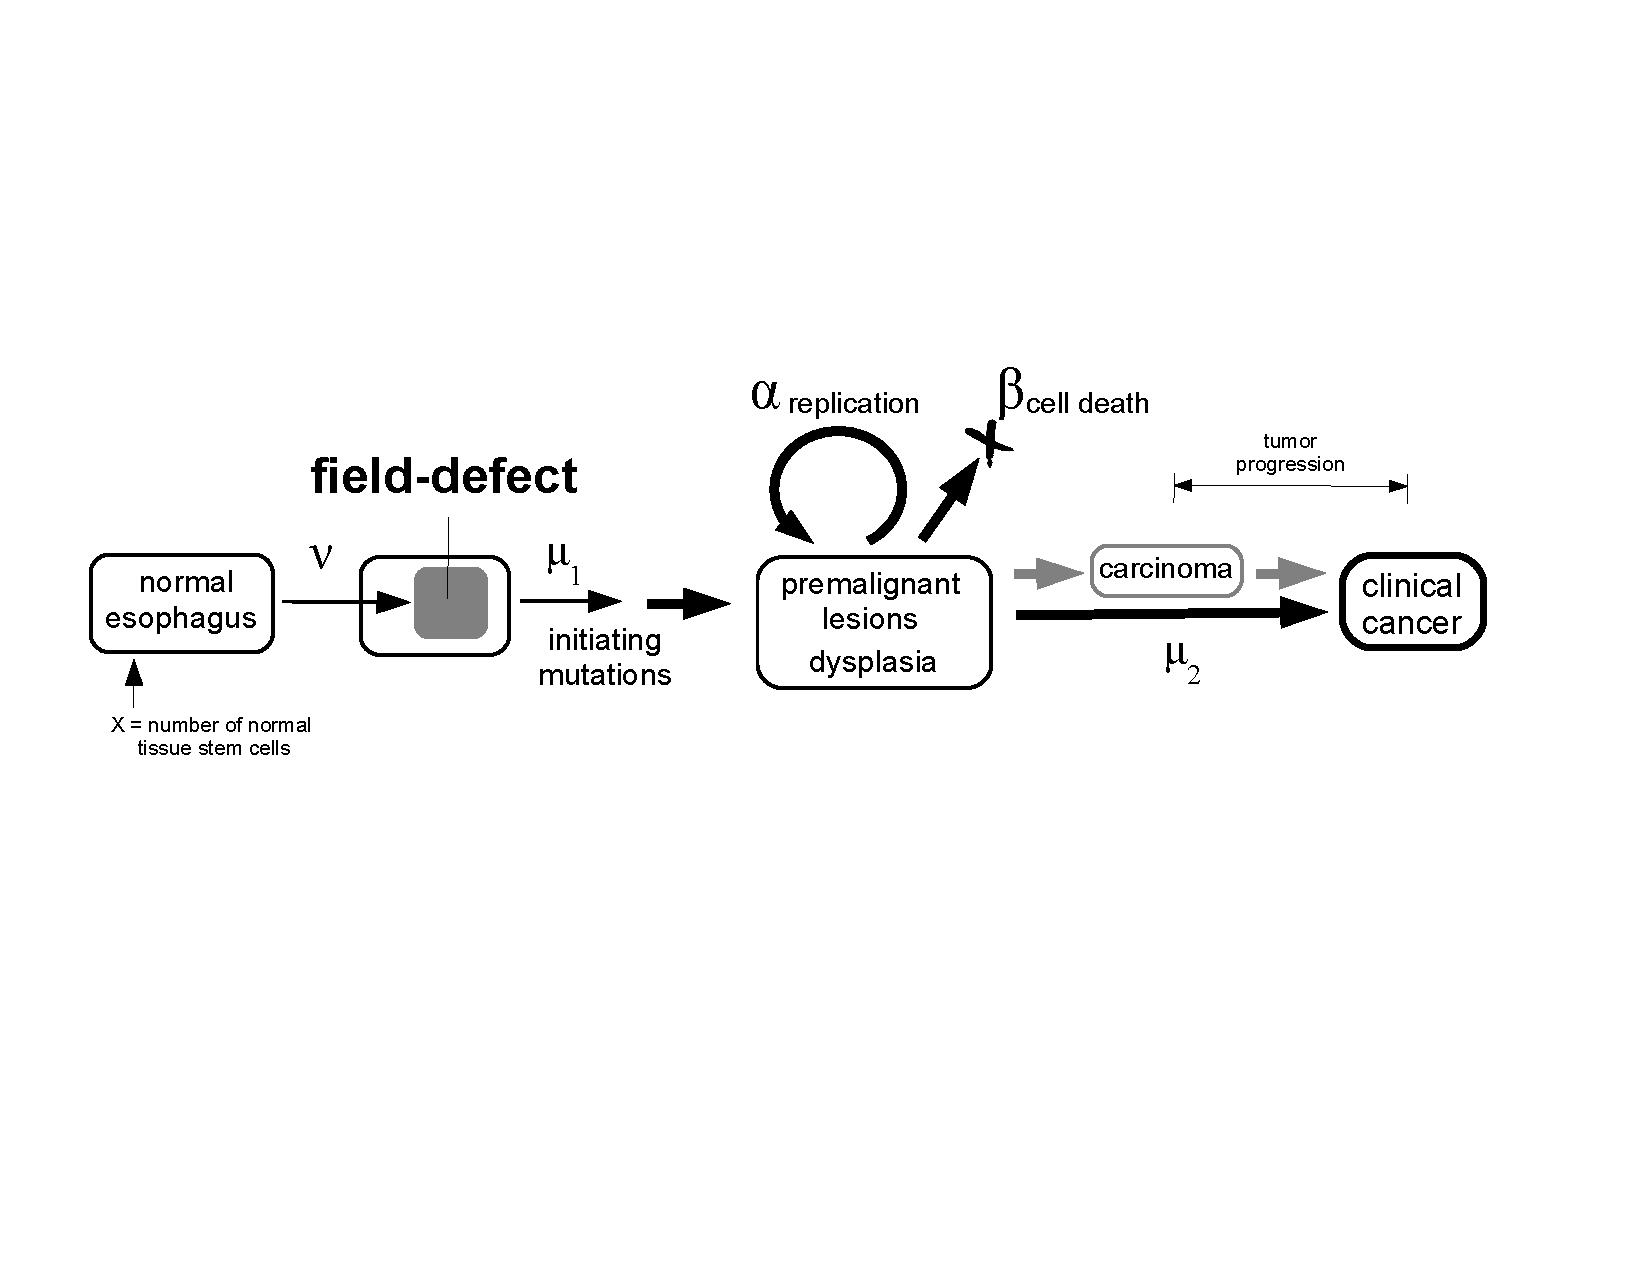
\includegraphics[scale=0.6, trim=0 0 0 0]{FEFF-model-2.pdf}
\caption{{\bf Multistage Clonal Expansion (MSCE) model for ESCC.} Model parameters are: $\nu$ the rate of an ESCC predisposing field-defect, $\mu_1$ the mutation rate (per field) for the initiation of premalignant (dysplastic) clones, $\alpha$ the cell division rate, $\beta$ the cell death rate, and $\mu_2$ the rate of malignant transformations. See text for further details.}
\label{fig1}
\end{adjustwidth}
\end{figure}

The mathematical derivation of the {\it hazard function}, $h(a)$, which is the rate at which cancers occur in a population of individuals who have not yet developed the cancer of interest by age $a$ (also known as {\it age-specific cancer incidence}), has been derived previously (e.g., ~\cite{Jeon2006}). Briefly, for the model depicted in Fig~\ref{fig1}, the hazard function can be written as a convolution of a random event that leads to a premalignant field and a subsequent process representing a two- or three-stage clonal expansion model which begins with initiating mutations that occur in cells that belong to the premalignant field:

\begin{eqnarray}
\label{eq:hazard}
    h(t) = \frac{\int_0^t ds \ f_{FD}(s)\ f_{MSCE}(t-s)}{1-\int_0^t ds \ f_{FD}(s)(1-S_{MSCE}(t-s))} 
\end{eqnarray}
where $f_{FD}(s) = \nu(s) e^{-\int_0^s dv \ \nu(v)}$ is the density function for the premalignant field-defect event. Note, when the FD rate $\nu$ is constant, this density function is strictly exponential. $S_{MSCE}(t-s)$ is the (tumor) survival function for the MSCE model component shown Fig~\ref{fig1}. Note, $f_{FD}(s)$ may be ``improper" if the hazard rate $\nu(s)$ vanishes at some time $s< \infty$, i.e., not all individuals may ever develop the field-defect. For a two-stage clonal expansion model (i.e., a single initiating mutational event is required to induce dysplastic cell proliferation), we have

\begin{eqnarray}
\label{eq:MSCE}
    f_{MSCE}(u) &=& h_2(u)\ S_2(u)
\end{eqnarray}
with    
\begin{eqnarray}
\label{eq:h2}
    h_2(u) = \frac{\mu_1}{\alpha} \frac{q p\ (e^{-q u}-e^{-p u})}{q e^{-p u}-p e^{-q u}}
\end{eqnarray}
and
\begin{eqnarray}
\label{eq:S2}
    S_2(u) = e^{-\int_0^u dv \ h_2(v)} = \big( \frac{q-p}{qe^{-pu}-pe^{-qu}} \big) ^{\mu_1/\alpha}
\end{eqnarray}
with
\begin{eqnarray}
\label{eq:pq}
    p &=& \frac{1}{2} \big( -\alpha+\beta+\mu_2 -\sqrt{(\alpha+\beta+\mu_2)^2 -4\alpha\beta} \big) \\ \nonumber
    q &=& \frac{1}{2} \big( -\alpha+\beta+\mu_2 +\sqrt{(\alpha+\beta+\mu_2)^2 -4\alpha\beta} \big) .
\end{eqnarray}
Rather than fitting the model parameters $p$ and $q$, we use the combinations $g=-(p+q)=\alpha-\beta-\mu_2$ (net cell proliferation) and $pq=-\alpha\mu_2$ ($\approx$ malignant transformation). The premalignant cell division rate $\alpha$ is non-identifiable from incidence data. To guarantee the identifiability of all other parameters we assumed $\alpha=17.4$/yr, the cell division rate for esophageal stem cells estimated by Tomasetti and Vogelstein~\cite{Tomasetti2015} for normal esophagus. Analogous expressions for a convolution of a field-event and a three-stage clonal expansion process are provided in Jeon et al.~\cite{Jeon2006}. 

\subsection*{Regularized age-period-cohort (APC) model}
Secular trends in cancer incidence data can be modeled using a traditional {\it proportional hazards} approach which assumes multiplicativity of the unadjusted hazard function (age effect) and associated period and cohort effects. A limitation of this approach is that the period effect ascribes incidence trends by year of diagnosis rather than by historical time. Here we introduce an alternative method which incorporates historic trends directly into the carcinogenesis process. 

To capture historic trends that affect the incidence rate of a premalignant field-defect, $\nu$, we simply allow $\nu$ to depend on age $s$ and birth year. Thus, given a birth cohort $B$, $\nu$ is also a function of calendar year $y$ by virtue of the relationship $y$ = $B+s$. Assuming that the field-defect has low probability of occurring early in life, we may also moderate this period trend with a term that forces $\nu \rightarrow 0$ below an age $s_0$, as shown in Fig~\ref{fig2}. This assumption can be relaxed, i.e. the logarithmic term $\log(s/s_0)$ in the shape function $f(y-y_0;s) = \log(\nu)$ can be omitted (see Fig~\ref{fig2} for definitions). However, we found significantly better fits by deviance for Blacks (both sexes) and white females with this term included ($ p < 2\cdot  10^{-4}$; $\tilde{\chi}^2 (1 \ df)$), which led to a more pronounced early increase in the field-defect rate $\nu(s)$. For white males, the fit only improved marginally. Furthermore, $\nu$ may also be influenced by effects that are strongly associated with birth cohort $B$, which we model using a multiplicative factor $\exp \big[b_1 (B-B_0)^2(1+b_2(B-B_0))\big]$, where $B_0$ is a reference birth year. Note, at time $B_0$ the modelled birth cohort effect has a zero derivative, therefore approaches unity (no effect) smoothly (Fig~\ref{fig2}). 

Finally, because general time trends may also affect rate of cancer progression, we also investigated whether the growth of dysplastic clones (within the premalignant field) shows significant trends by birth cohort. To this end, we imposed a simple linear-quadratic birth-cohort adjustment on the promotion parameter $g=\alpha-\beta-\mu_2$ of the form:
$$g=g_0 \exp{g_1(B-1800)(1+g_2(B-1800))},$$
where $B$ is the birth year, as above.  
\medskip
\begin{figure}[!ht]
\begin{adjustwidth}{-1in}{0in} 
% Comment out/remove adjustwidth environment if table fits in text column.
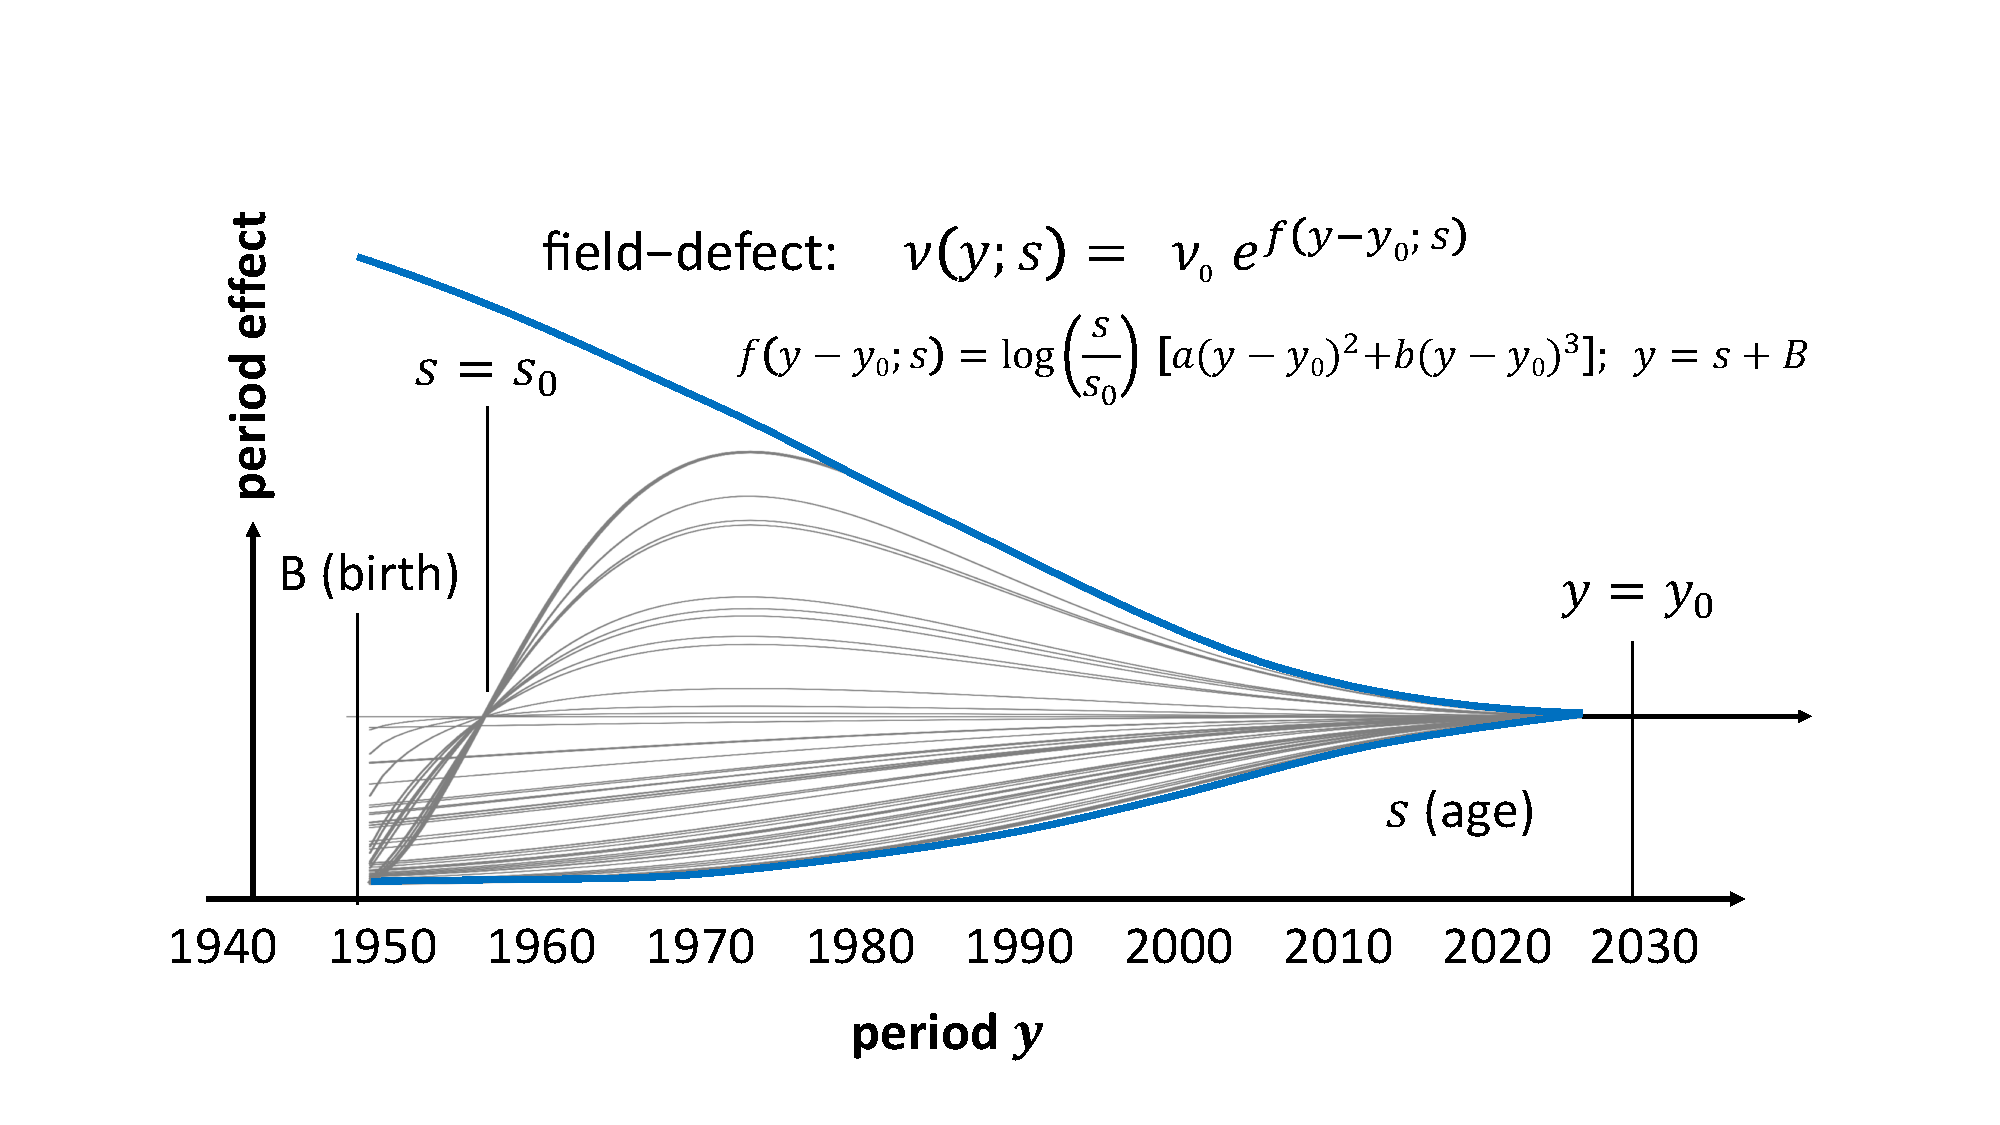
\includegraphics[scale=0.5, trim=0 0 0 0]{Fig2.pdf}
\end{adjustwidth}
\caption{{\bf Functional regularization of period (year) trends on the field-defect rate $\nu$.} Note, $\nu$ approaches the background rate $\nu_0$ smoothly at some reference point $y_0$. Here $s$ refers to age, $B$ to birth year, $y$ to period.}
\label{fig2}
\end{figure}

% For figure citations, please use "Fig" instead of "Figure".
% \nameref{S1_Video} 
% Place figure captions after the first paragraph in which they are cited.

% Results and Discussion can be combined.
\section*{Results}
Here we present findings related to the main biological processes that shape the age-specific incidence of ESCC by sex and race in the US, and how parameters that control these processes are modulated by period and cohort effects. Our analysis follows previous work for colorectal cancer and esophageal adenocarcinoma, but uses the new computational approach outlined in Methods for estimating the impact of period and cohort effects on the biological model parameters.
\subsection*{ESCC field cancerization}
We first conducted preliminary analyses of ESCC incidence data from the SEER9 registry (years 1975-2016; birth cohorts $\leq 1960$) using a multistage clonal exapnsion (MSCE) model that assumes that normal (tissue) stem cells need to acquire 2 driver mutations before they undergo stochastic clonal growth ~\cite{Luebeck2013} (see Fig~\ref{fig3}A). Period and cohort adjustments were performed as previously described. The best model fits (by deviance) were obtained using the regularized period and cohort adjustments acting on the first mutational event (rate $\mu_0$) for the model in which normal stem cells are considered as independent and at equal risk of generating progeny that give rise to cancer. Alternatively, we explored a model that stipulates a multi-cellular field-defect with rate $\nu$ as the first event (see Fig~\ref{fig3}B). 
\medskip
\begin{figure}[!ht]
\begin{adjustwidth}{0.25in}{0in} % Comment out/remove adjustwidth environment if table fits in text column.
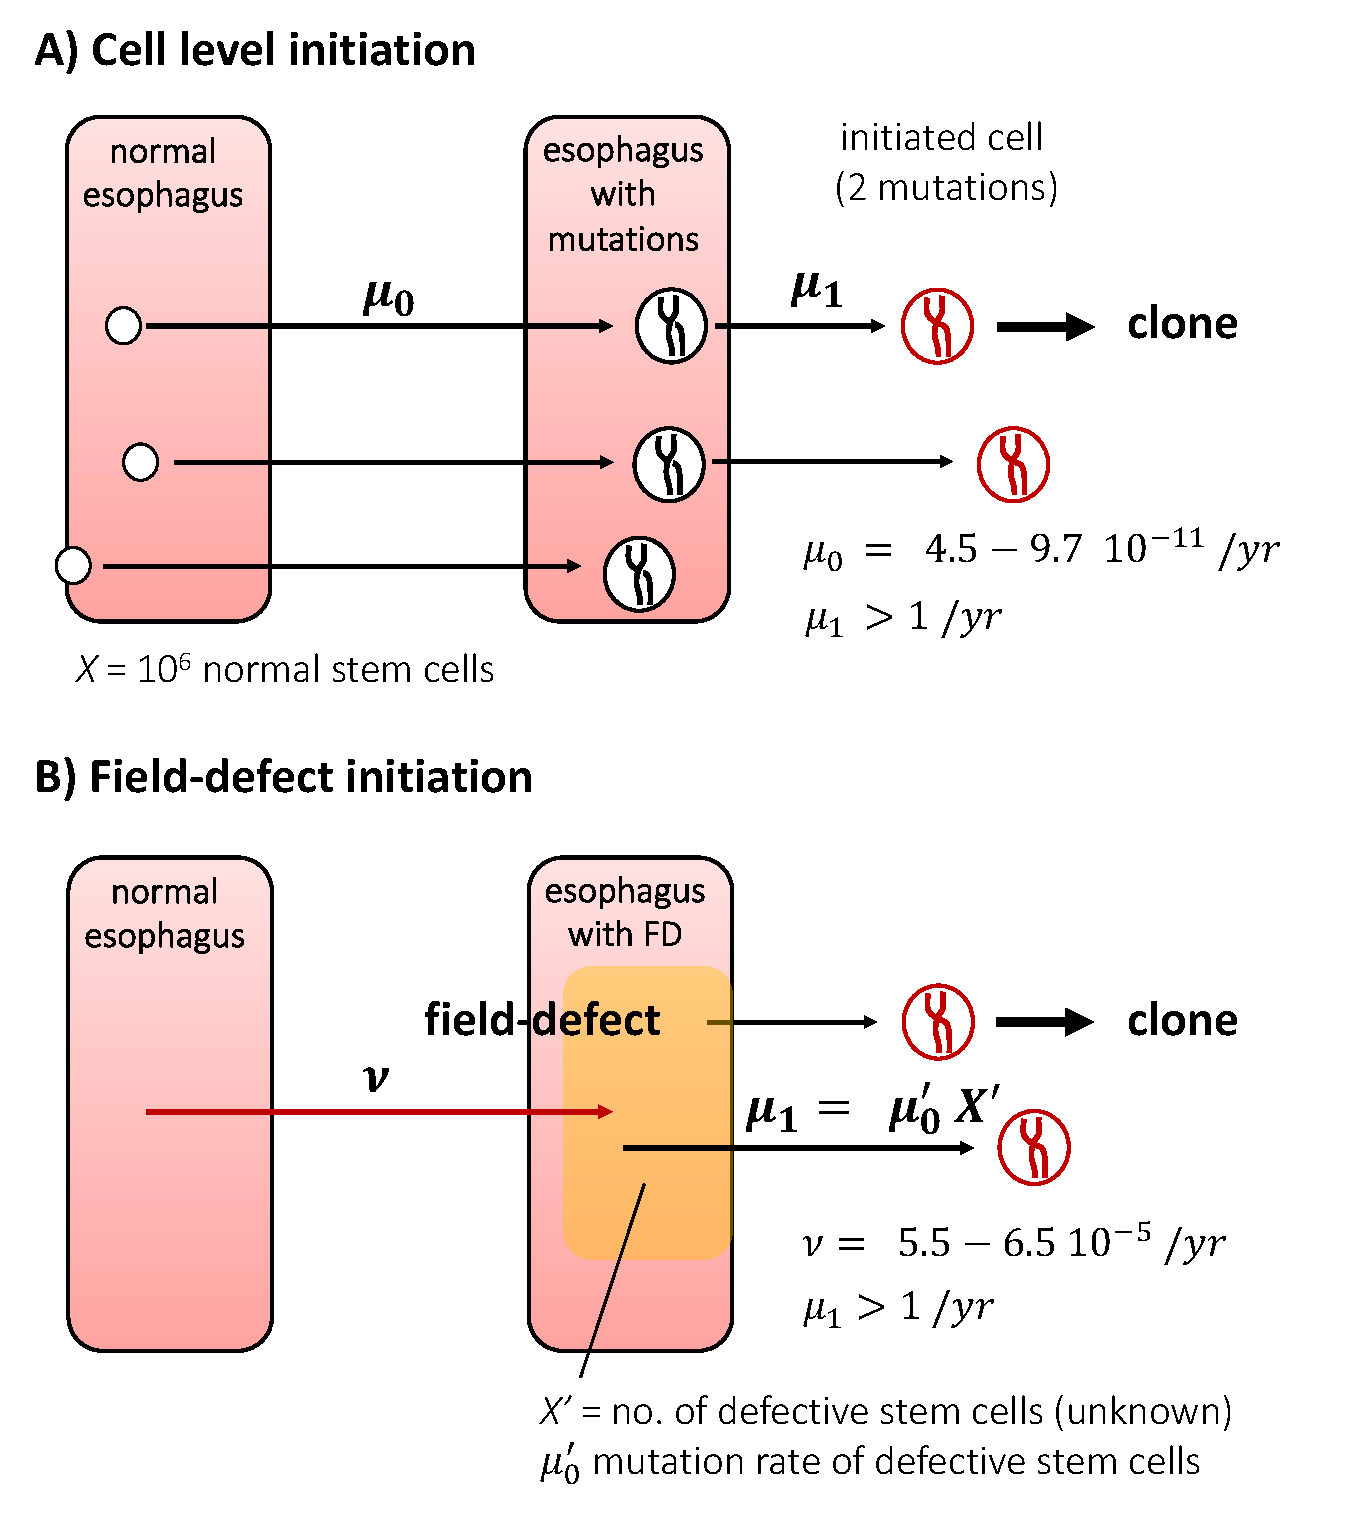
\includegraphics[scale=0.5, trim=0 0 0 0]{Fig3.pdf}
\caption{{\bf A) Two-hit process for the initiation of dysplastic clones; B) Sporadic formation of field-defect followed by single hit process for the initiation of dysplastic clones. Note, only the product $\mu_1=\mu_0'X'$ is identifiable and represents the rate at which dysplastic clones are initiated in the defective field.}}
\label{fig3}
\end{adjustwidth}
\end{figure}

Maximum likelihood analyses with the two models provided similar fits to the ESCC incidence data. However, only the FD model yielded biologically plausible parameter estimates for the rates of mutations that lead to premalignant clones (see Fig~\ref{fig3}). We arrived at this conclusion via the following reasoning: 1) in the absence of a field-defect all normal tissue stem cells are at risk of acquiring the first rate-limiting mutation with rate $\mu_0$ per cell. Assuming the the human esophagus has about $10^6$ normal stem cells~\cite{Tomasetti2015}, each of which is at risk to acquire the first requisite driver mutations, we estimated $\mu_0$ to be in the range of 4.5-8.7 $10^{-11}$ per year for both sexes and races (Blacks and Whites) - mutation rates which are much smaller than the rate of sporadic DNA base substitutions, especially considering that most stem cells divide numerous times per year. More importantly, 2) estimates of the second rate-limiting mutation, $\mu_1$, were exquisitely high for all groups, i.e. $> 1$ per year (Table 1), which suggests a large number of cells make up the field-defect since $\mu_1$ may be considered the product of a (large) number of stem cells within the field and a (small) locus-specific mutation rate per cell. Locus-specific mutation rates are known to vary with gene size and function, but are generally assumed to be in the range of $10^{-4}$ to $10^{-5}$ per year~\cite{Drake1998}, depending on the rate of stem cell divisions. Thus, the field-defect, once established, appears to entail a large ($>10^4$) number of normal stem cells. Thus, a model that assumes that all normal esophageal stem cells are at equal risk to transform into a clinical esophageal malignancy did not yield plausible biological rates. However, excellent fits to incidence data along with biologically plausible rates were found when using a model where a large number of cells first establish a permissive field of activated cells that are prone to stochastic initiation of dysplasia.
% We also allowed for a third rate-limiting mutation to occur before clonal expansions can occur, but found no improvements in model fits. 

\subsection*{ESCC incidence by age group and calendar year}
ESCC incidence rates show remarkable differences by sex and race (black and white SEER9 population) and by calendar year (i.e., year of ESCC diagnosis), as seen in Fig~\ref{fig4}. Especially striking is the $\sim 4$-fold higher incidence of ESCC in the 1980's for black males and their decline to levels still much above the current incidence levels among white males. Although black males and females differ in overall levels they share rather similar curvatures for all three age groups shown in Fig~\ref{fig4}. In contrast, the patterns for white males and females differ visibly, especially for the older age group (70+). The ESCC incidences for white males stand out from the others in that they appear to decline monotonically, showing virtually no curvature for the period 1975-2016 for which we have data, with incidence levels that approach those of white females in earlier years.
\medskip
\begin{figure}[t]
\begin{adjustwidth}{-2.in}{0in} % Comment out/remove adjustwidth environment if table fits in text column.
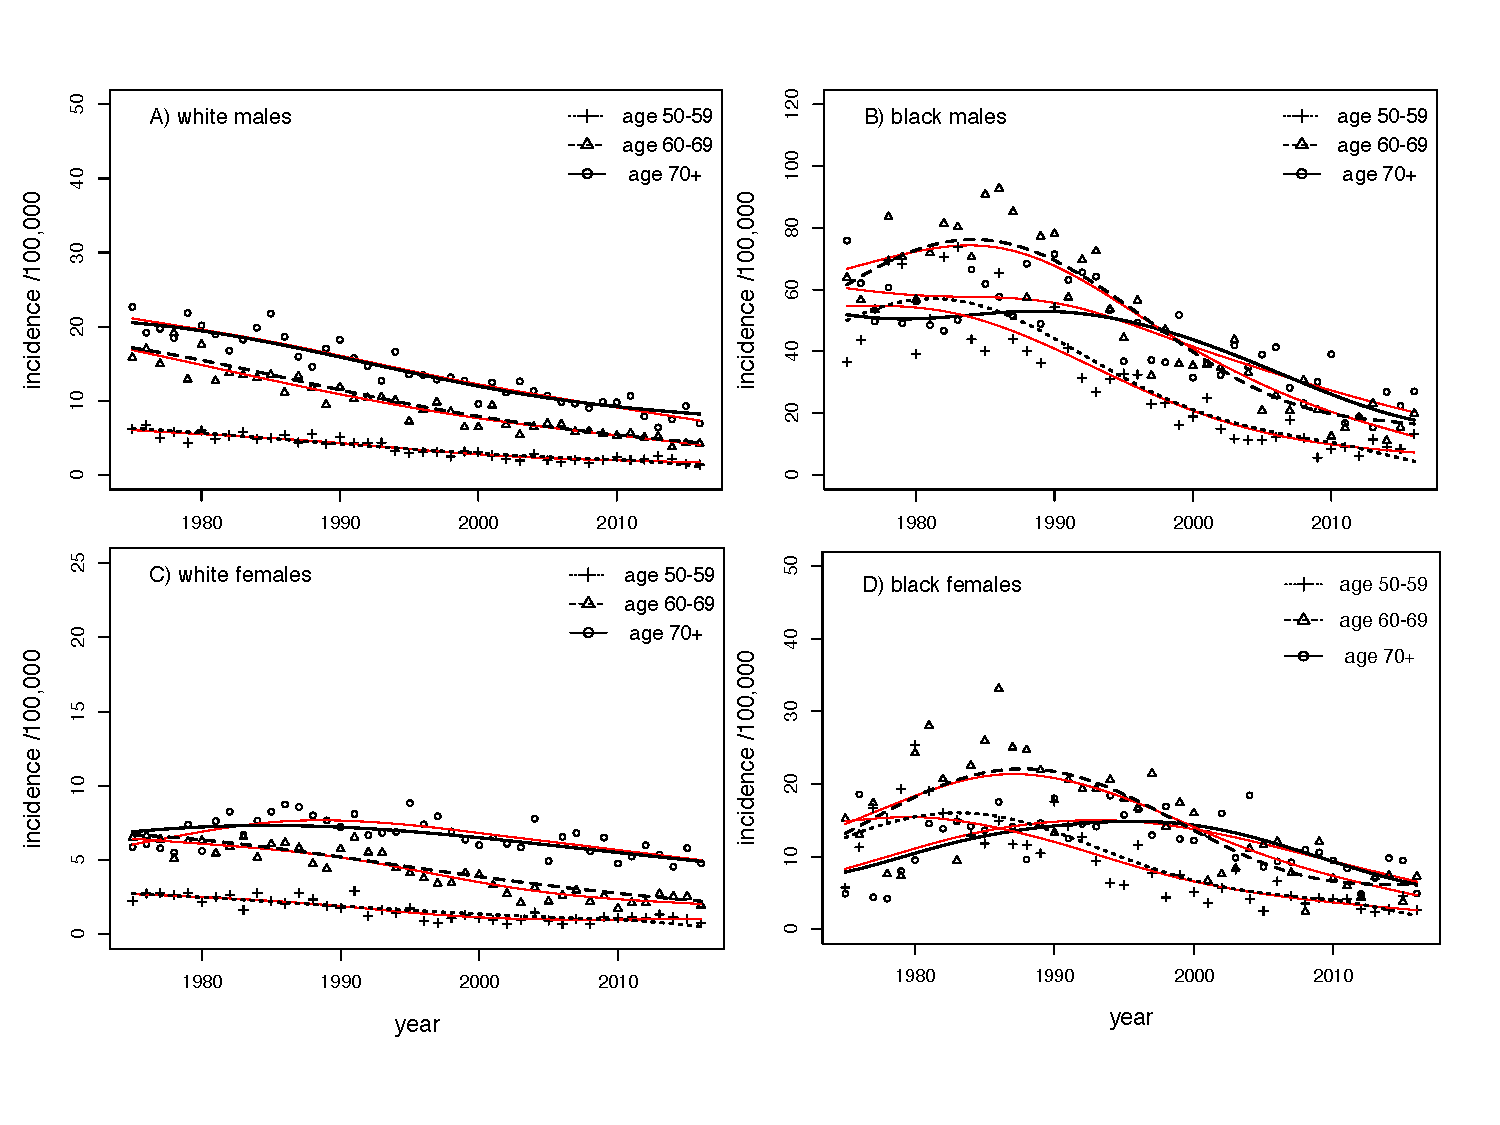
\includegraphics[scale=0.7, trim=0 20 0 50]{AgeSpec_Incidence_by_CY_SEER9-2016_panel.pdf}
\caption{{\bf ESCC incidence (data, black shapes; model fits, black lines) by sex, race and age group as indicated from 1975-2016. For comparison, non-parametric fits using $4^{th}$-order smoothing splines are shown in red.}}
\label{fig4}
\end{adjustwidth}
\end{figure}

\subsection*{The influence of historic period and birth-cohort on the risk of developing an esophageal field-defect}
As described in Methods, the regularized model for ESCC incorporates both period and cohort effects. Our model fits (Fig~\ref{fig5}, Table~1) show that the age-specific rate at which a premalignant field-defect is induced in the esophagus prior to the development of cancer is strongly affected by age and historical period. Fig~\ref{fig5} shows the predicted influence on the field cancerization rate $\nu(s; B)$ as a function of period (i.e. historic time from the late 1800's to the year 1980) for fixed birth cohorts $B$, as indicated.  

The emerging (estimated) time profiles for the field-defect rate $\nu(s)$ show surprisingly narrow time distributions (about 5-6 years for Blacks, about 10 years for Whites) with their maxima at $<10$ years. These curves also differ remarkably between the races (Fig~\ref{fig4}). For black men and women, we see very similar cohort patterns in that the presumed field-defect rate is predicted to peak sharply in the first decade of life. For Whites, the predicted rate curves are somewhat wider with their maximum between ages 5 and 10, well before smoking initiation would begin~\cite{Holford2016}.  Note that the estimated period effect for $\nu(s; B)$ among white males is qualitatively distinct from the other groups in that the cohort-specific maxima of $\nu(s; B)$ decline monotonically as seen in Fig~\ref{fig5}.
\medskip
\begin{figure}[t]
% \begin{adjustwidth}{-2.25in}{0in} % Comment out/remove adjustwidth environment if table fits in text column.
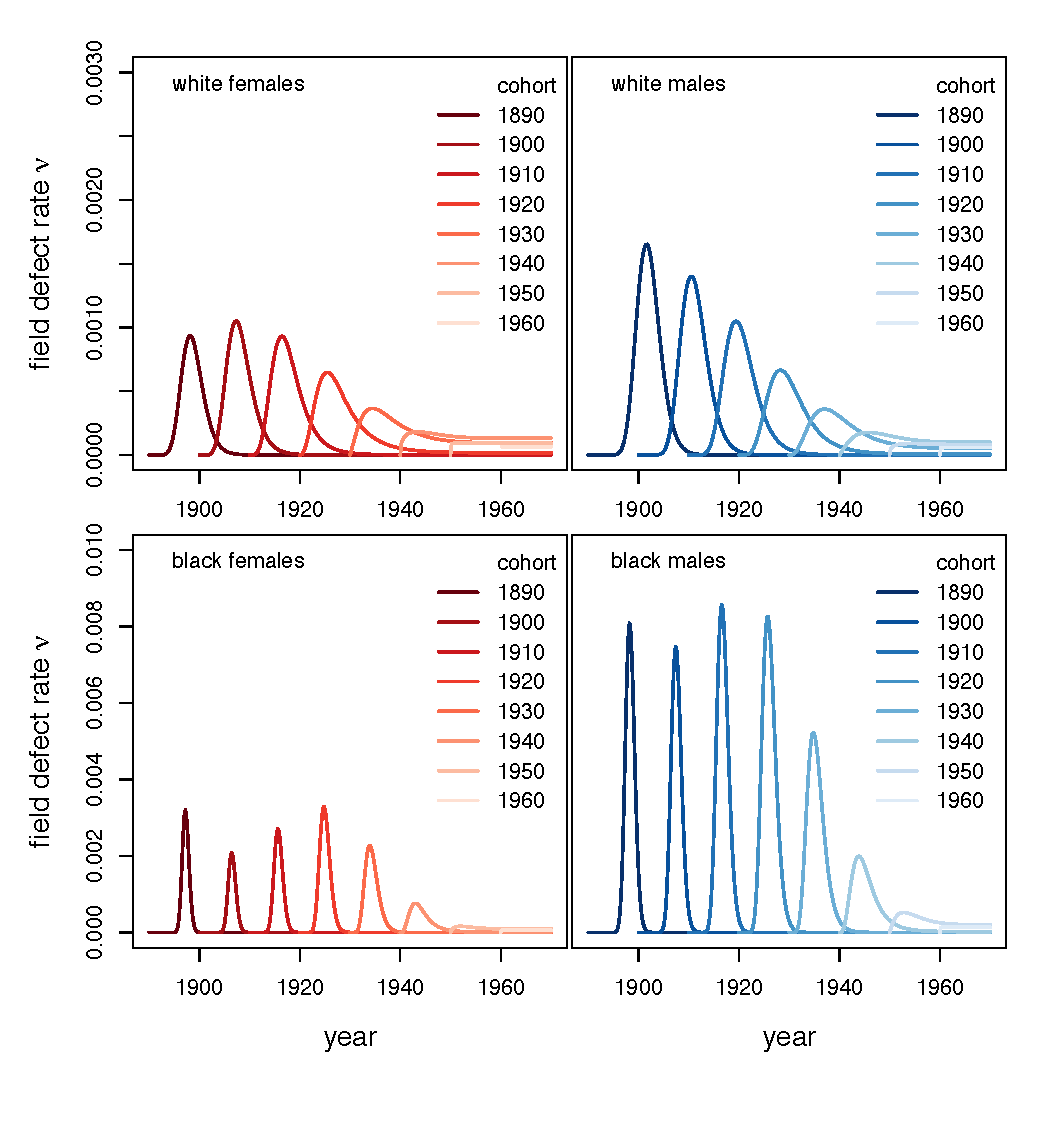
\includegraphics[scale=0.8, trim=0 0 0 40]{FEFFrates_SEER9-2016_panel.pdf}
\caption{{\bf Period profiles of the field-defect rate $\nu(s;B)$ by birth cohort as indicated.}}
\label{fig5}
% \end{adjustwidth}
\end{figure}
%The field-defect profiles shown in Fig~\ref{fig5} are generated by a multiplicative model for combining period and cohort effects as described in Methods.

Fig~\ref{fig6} shows the estimated field-defect rate $\nu(s; B)$ (panel A) and corresponding age-specific FD prevalence (panel B) for the 1920 cohort among both sexes and races (analogous plots for other cohorts in shown in Fig S2). This comparison shows the dramatic differences in the maximal strength of the field-defect rate between the races. Beyond childhood, the predicted prevalences of the field-defect among black males is roughly 3-fold higher than for the other groups, approximately 3$\%$.     

\subsection*{Birth cohort effects on premalignant cell proliferation (promotion).}
For Blacks (both sexes), we find significant increasing birth-cohort effects on the promotion parameter $g$ ($\tilde{\chi}^2$(2 df) $p<5\cdot 10^{-5}$), assuming a null hypothesis with no trends ($g_1=g_2=0$) . Similar for white females ($p< 10^{-3}$). However, for white males, we found no significant birth cohort effect on promotion. S1 Fig shows the cell proliferation (promotion) parameter $g$ as a function of birth cohort for all 4 populations analyzed.
% For whites females we obtain lightly better fits assuming cohort effects on the initiation rate $\mu_1$ compared with an effect on the promotion rate $g$.

\medskip
\begin{figure}[t]
% \begin{adjustwidth}{-2.25in}{0in} % Comment out/remove % Comment out/remove adjustwidth environment if table fits in text column.
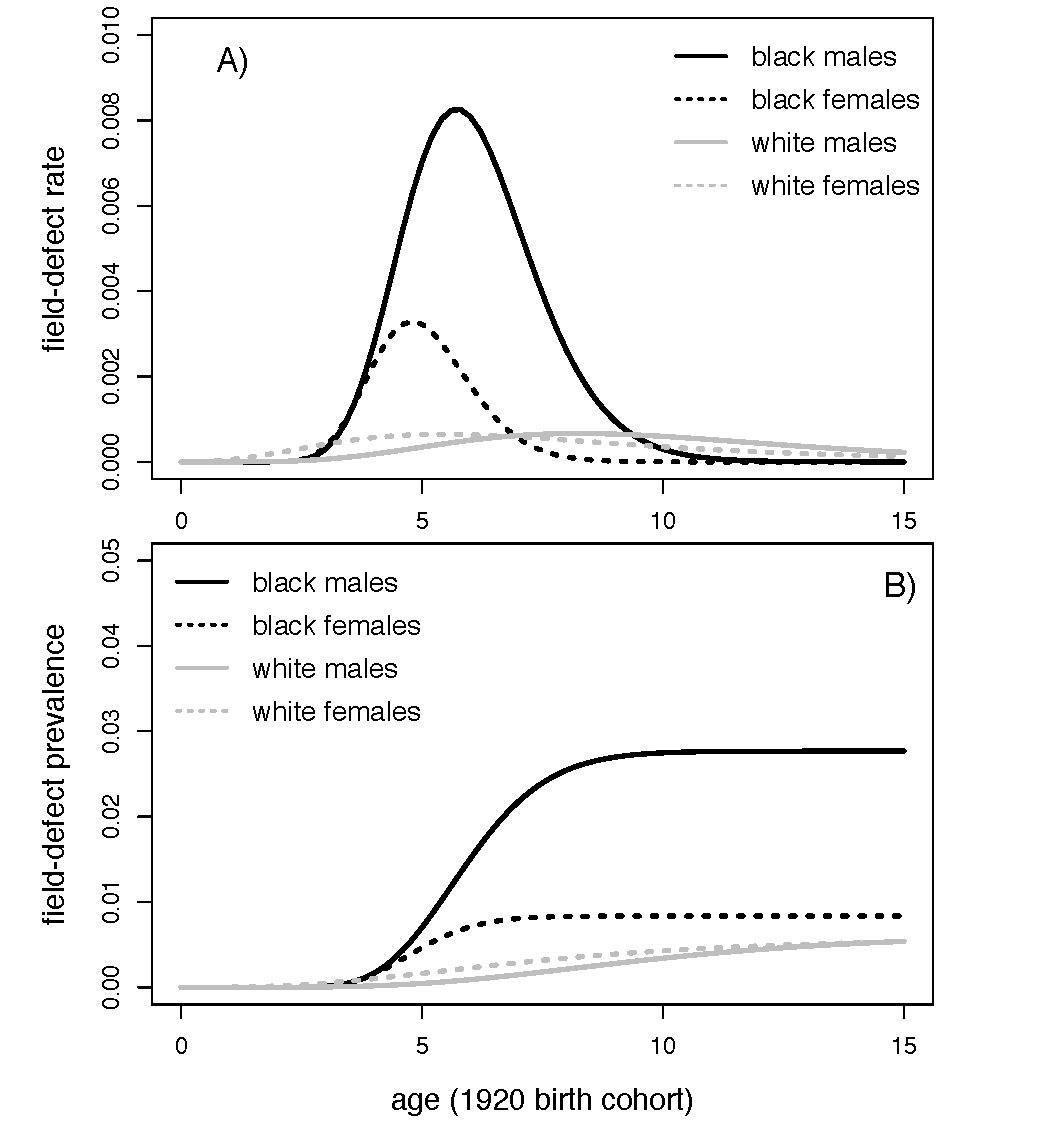
\includegraphics[scale=0.7, trim=0 0 0 0]{Fig6.pdf}
\caption{{\bf Predicted field-defect rates $\nu$ (panel A)} and corresponding field-defect prevalences as functions of age (1920 birth cohort) by race and sex.}
\label{fig6}
% \end{adjustwidth}
\end{figure}

\section*{Discussion}

Although the origin of ESCC has previously been associated with field cancerization involving both epigenetic and genetic defects that give rise to multifocal dysplasia in esophageal and other tissues ~\cite{Slaughter1953,  Ohashi2015}, the clinical evidence is scant and may be confounded with the ubiquitous presence of driver mutations ({\it TP53, Notch1}) in normal squamous tissue ~\cite{Martincorena2018}. Surprisingly, this analysis of ESCC incidence patterns using a mathematical model that integrates the main cellular processes involved in cancer development, suggests that the known advanced precursor to ESCC (i.e. esophageal dysplasia) arises within a premalignant field that primarily develops early in life and is under the influence of strong historic trends. Although environmental exposures, such as cigarette smoking, alcohol consumption may contribute to field formation later in life, the young-age signatures and time trends of the inferred premalignant field-defect suggest that other factors such as pediatric malnutrition and vitamin deficiencies may significantly influence ESCC incidence patterns in the US.

Whether nutrition or other factors, this study suggests that there is a critical early-childhood window of susceptibility for developing field-defects that predispose to the later development of ESCC. While our exploration of the SEER-based ESCC incidence data~\cite{SEER2019} reveal the known strong disparities of ESCC rates between Blacks and Whites~\cite{Brown2001}, our results also suggest that there is a significantly higher risk for developing field-defects during childhood for Blacks than for Whites, especially among the earlier birth cohorts when nutritional or other disparities may have been more prevalent among Blacks. Other predisposing factors for ESCC include the possible impact of pathogens such as Human Papilloma Virus (HPV) \cite{Dinc2020} and interactions of the microbiome with evolving dietary patterns. 

Our conjecture that the carcinogenic process for ESCC mainly begins with the development of a field-defect rather than with sporadic rare mutations in individual stem cells is based on the comparison shown in Fig~\ref{fig3}. Both scenarios (cell-level vs FD initiation) fit the ESCC incidence patterns equally well but differ in terms of the hazard function and estimated model parameters as discussed under {\it ESCC field cancerization}. Importantly, the sporadic (independent) stem cell mutation scenario (Fig~\ref{fig3}A) yields mutation rates that are implausible while the FD scenario yields estimates that are in line with the concept of an abnormal (defective) esophageal tissue in which rare (rate-limiting) mutations lead to the initiation of dysplasia. Since mutations in TP53 are found in virtually all ESCC \cite{Agrawal2012, TCGAeso2017}, it is plausible to assume that the first mutation in the field-defect involves loss of TP53 tumor suppressor function followed by a malignant transformation in response (or due) to the biallelic loss of TP53 control consistent with Knudson's two-hit model \cite{Knudson1973}. However, the molecular nature of the conjectured field-defect is unclear but has been associated with epigenetic alterations associated with smoking and alcohol consumption confounded by other factors such as low BMI and poor diet~\cite{Lee2011}. 
%Furthermore, our findings suggest that for older cohorts the carcinogenic effectiveness of the field-defect was transient, lasting \~10 years and occurred quite early in life (see Results). 

% Our findings add an important piece of information to the plethora of recognized risk factors for ESCC. Beyond smoking and excess alcohol consumption and their synergistic interactions \cite{Pandeya2009}, malnutrition, vitamin deficiencies and genetic predispositions~\cite{Matejcic2019, Canova2010} have also been implicated as risk factors. Further dietary items include hot liquids \cite{Liu2019} and salty meats \cite{Lin2015}. Other recognized risk factors that occur less frequently include achalasia, a chronic inflammatory condition where food collects in the lower esophagus \cite{Nesteruk2019}, tylosis - a rare autosomal dominant proliferative skin disease associated with very high risk of ESCC \cite{Hosur2018}, and Plummer-Vinson syndrome (PVS), an extremely rare condition characterised by iron deficiency anaemia and increased risk for ESCC \cite{Novacek2006}, as well as infection of esophageal lesions with HPV \cite{Dinc2020} and recent occurrence of head and neck cancers \cite{Tseng2020}.

In summary, our findings suggest the disparate demographic patterns observed in the US may not be wholly attributable to smoking and alcohol, but may also reflect other factors acting early in life. This conclusion is supported by the similarity of recently re-assessed historic smoking initiation and prevalence distributions in the US between Whites and Blacks \cite{Holford2016}. Modest differences in smoking and alcohol use alone may therefore not fully explain the high degree of racial divergence and recent converging trends in ESCC incidence between Whites and Blacks. Environmental exposures, such as cigarette smoking, alcohol and industrial exposures may well contribute to field formation later in life (and increased promotion of precursor lesions), however the young-age signatures and time trends of the inferred premalignant field-defect suggest that other factors such as pediatric malnutrition, iron deficiency anemia (IDA) and deficiencies of some B vitamins (e.g. riboflavin, thiamin) may more significantly be involved in shaping the historic ESCC incidence patterns in the US~\cite{Taylor2013,Abnet2018}. 

% \section*{Conclusion}

% CO\textsubscript{2} 
% xxxx \nameref{S1_Appendix}.
\newpage
\noindent
ParameterParameter estimates are based on posterior samples obtained via Markov Chain Monte Carlo (MCMC) using random uniform prior distributions with boundaries that were well outside the obtained 95\% confidence regions. For sampling we used a multivariate Metropolis-Hastings algorithm with $>100,000$ samples for Males and $>200,000$ samples for Females. 

% test Table
\begin{table}
\begin{adjustwidth}{-1.5in}{0in} 
\caption{\label{tab:} A: marginal posterior medians (Blacks) with 95\% confidence regions}
\centering
\begin{tabular}[t]{l>{\bfseries\leavevmode\color{black}}rrr>{\bfseries\leavevmode\color{black}}rrr}
\toprule
\multicolumn{1}{c}{parameter} & \multicolumn{3}{c}{Black Males} & \multicolumn{3}{c}{Black Females} \\
\cmidrule(l{3pt}r{3pt}){1-1} \cmidrule(l{3pt}r{3pt}){2-4} \cmidrule(l{3pt}r{3pt}){5-7}
  & median & lower & upper & median & lower & upper\\
$\nu_0$ ($\times 10^{-5}$) & 9.54 & 8.06 & 11.4 & 5.52 & 4.38 & 7.12 \\
$\mu_1$ & 39.4632 & 27.5652 & 55.3248 & 15.7833 & 7.9030 & 30.8817\\
$\mu_2$ ($\times 10^{-7}$) & 0.0345 & 0.0087 & 0.1009 & 0.4878 & 0.0974 & 1.8217\\
$g_0$ & 0.0249 & 0.0210 & 0.0296 & 0.0632 & 0.0443 & 0.0928\\
$g_1$ & 0.0268 & 0.0248 & 0.0296 & 0.0096 & 0.0057 & 0.0136\\
$g_2$ & -0.0029 & -0.0032 & -0.0028 & -0.0011 & -0.0022 & -0.0003\\
\addlinespace
$b_1$ & 0.0106 & 0.0103 & 0.0111 & 0.0139 & 0.0132 & 0.0149\\
$b_2$ & 0.0440 & 0.0436 & 0.0443 & 0.0610 & 0.0589 & 0.0640\\
$w_1$ & 0.0002 & 0.0002 & 0.0002 & 0.0011 & 0.0011 & 0.0012\\
$w_2$ & -0.7856 & -0.8194 & -0.7574 & -0.2582 & -0.2779 & -0.2435\\
$y_0$ & 1967.1696 & 1965.2571 & 1969.0098 & 1961.0000 & - & - \\
$s_0$ & 0.4954 & 0.4773 & 0.5133 & 0.3586 & 0.3150 & 0.3989\\
\bottomrule
\end{tabular}
\setcounter{table}{0}
\medskip
\caption*{\ \ \ \phantom{Table 1.} B: marginal posterior medians (Whites) with 95\% confidence regions}
\centering
\begin{tabular}[t]{l>{\bfseries\leavevmode\color{black}}rrr>{\bfseries\leavevmode\color{black}}rrr}
\toprule
\multicolumn{1}{c}{parameter} & \multicolumn{3}{c}{White Males} & \multicolumn{3}{c}{White Females} \\
\cmidrule(l{3pt}r{3pt}){1-1} \cmidrule(l{3pt}r{3pt}){2-4} \cmidrule(l{3pt}r{3pt}){5-7}
  & median & lower & upper & median & lower & upper\\
\midrule
$\nu_0$ ($\times 10^{-5}$) & 5.52 & 4.76 & 6.44 & 6.51 & 4.05 & 14.2 \\
$\mu_1$ & 4.3755 & 3.3452 & 5.5657 & 1.2988 & 0.4992 & 2.9233\\
$\mu_2$ ($\times 10^{-7}$) & 1.3273 & 0.7746 & 2.2392 & 0.3392 & 0.0602 & 1.0892\\
$g_0$ & 0.1836 & 0.1686 & 0.1998 & 0.2032 & 0.1670 & 0.2488\\
$g_1$ & 0.0001 & 0.0000 & 0.0010 & 0.0000 & 0.0000 & 0.0000\\
$g_2$ & 0.0688 & 0.0039 & 1.3313 & 14.5845 & 3.4146 & 43.1293\\
\addlinespace
$b_1$ & 0.0038 & 0.0033 & 0.0043 & 0.0042 & 0.0033 & 0.0053\\
$b_2$ & 0.0305 & 0.0295 & 0.0315 & 0.0289 & 0.0265 & 0.0331\\
$w_1$ & 0.0006 & 0.0005 & 0.0007 & -0.0002 & -0.0002 & -0.0001\\
$w_2$ & -0.0928 & -0.1057 & -0.0844 & 0.2786 & 0.2142 & 0.3670\\
$y_0$ & 1963.0811 & 1961.2545 & 1966.8300 & 1961.0000 & - & - \\
$s_0$ & 1.8121 & 1.4694 & 2.2899 & 0.6246 & 0.5059 & 0.8992\\
\bottomrule
\end{tabular}
\end{adjustwidth}
\end{table}

\newpage

\section*{Supporting information}

% Include only the SI item label in the paragraph heading. Use the \nameref{label} command to cite SI items in the text.
\paragraph*{\Large{S1 Fig.}}
\label{S1_Fig}
%\begin{figure}[!ht]
% \begin{adjustwidth}{-2.25in}{0in} % Comment out/remove % Comment out/remove adjustwidth environment if table fits in text column.
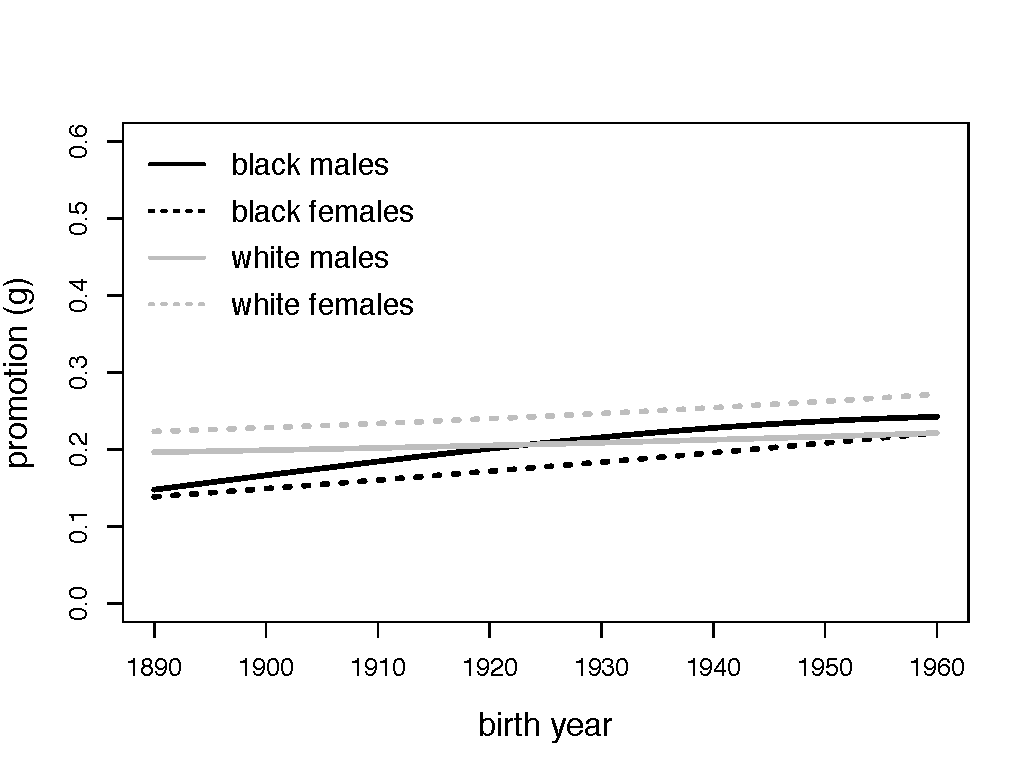
\includegraphics[scale=0.7, trim=0 0 0 0]{Promotion_g_SEER2016_by_BC.pdf}
% \end{adjustwidth}
%\end{figure}
{\bf Promotion.} Estimated cell proliferation parameter $g$ as a function of birth cohort.

\paragraph*{\Large{S2 Fig.}}
\label{S2_Fig}
%\begin{figure}[!ht]
% \begin{adjustwidth}{-2.25in}{0in} % Comment out/remove % Comment out/remove adjustwidth environment if table fits in text column.
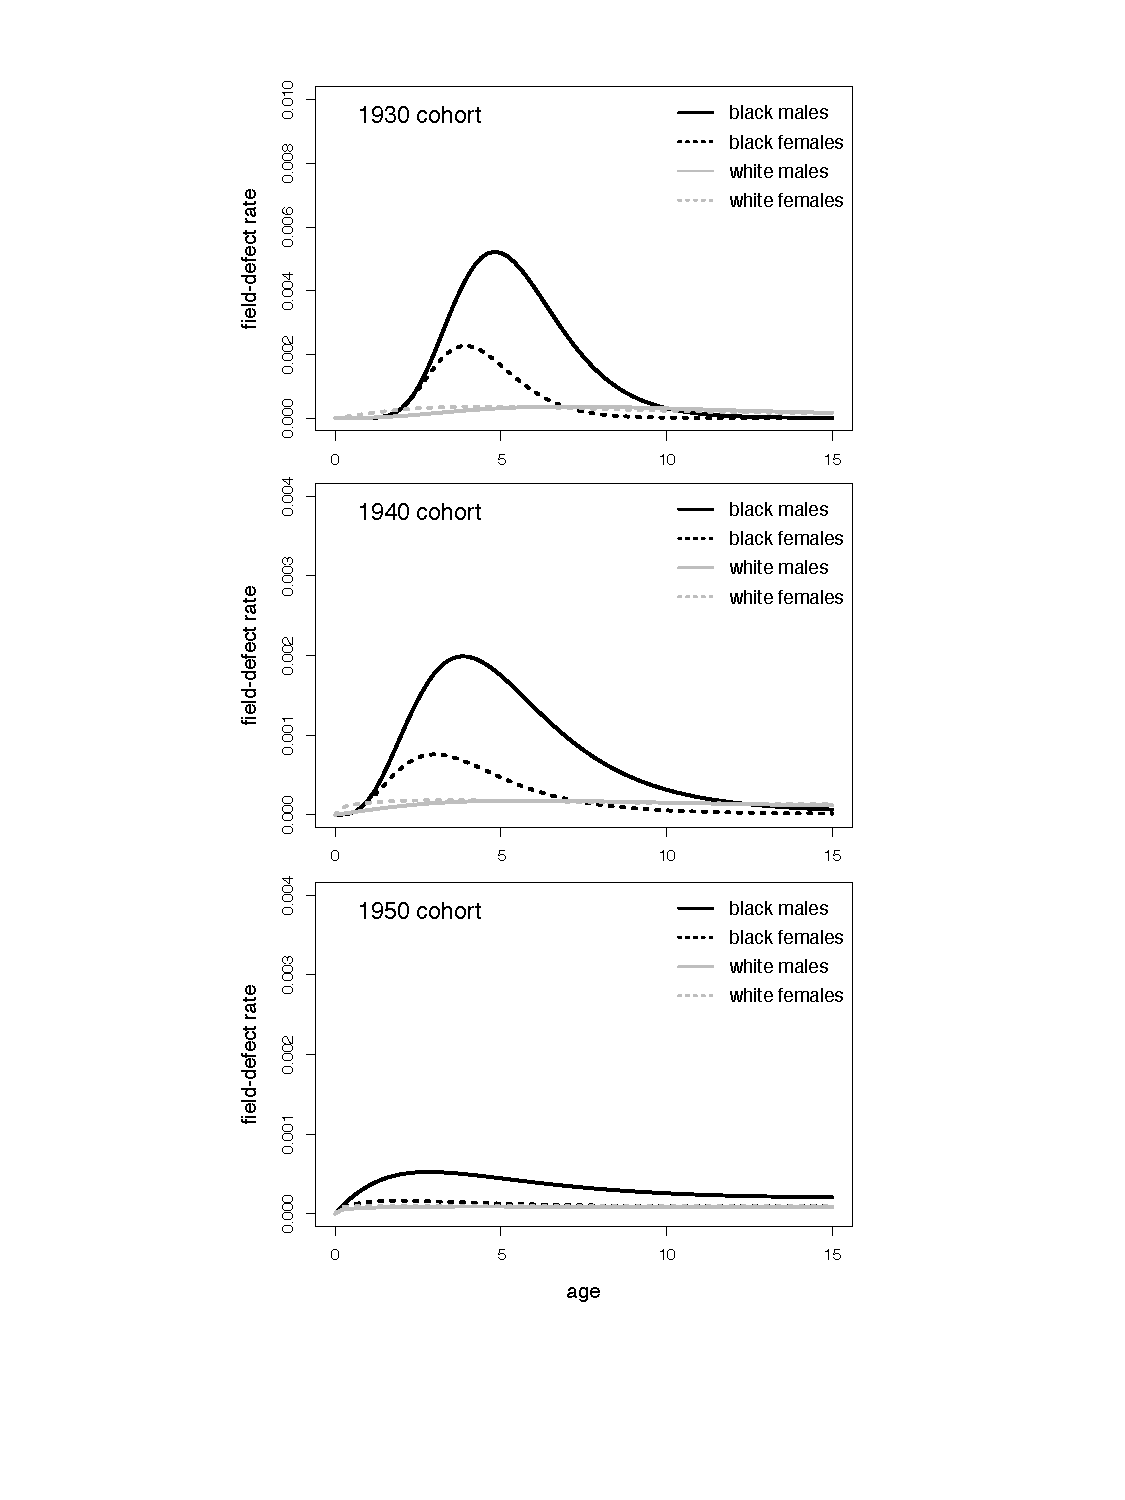
\includegraphics[scale=.85, trim=40 80 0 0]{S2 Fig.pdf}
% \end{adjustwidth}
%\end{figure}
{\bf ESCC Field-Defect Rates} for the 1930, 1940 and 1950 birth cohort for both sexes and races. 

\section*{Acknowledgments}
This research was supported by the National Cancer Institute (www.cancer.gov) grant U01CA152926 (CISNET) and by ...

\nolinenumbers

% Either type in your references using
% \begin{thebibliography}{}
% \bibitem{}
% Text
% \end{thebibliography}
%
% or
%
% Compile your BiBTeX database using our plos2015.bst
% style file and paste the contents of your .bbl file
% here. See http://journals.plos.org/plosone/s/latex for 
% step-by-step instructions.
% 

% Bibliography
%\begin{thebibliography}{10}
\bibliography{MyTeX}
%\end{thebibliography}

\end{document}


~\cite{bib1} 
Eq~(\ref{eq:schemeP}) 

\begin{eqnarray}
\label{eq:schemeP}
	\mathrm{P_Y} = \underbrace{H(Y_n) - H(Y_n|\mathbf{V}^{Y}_{n})}_{S_Y} + \underbrace{H(Y_n|\mathbf{V}^{Y}_{n})- H(Y_n|\mathbf{V}^{X,Y}_{n})}_{T_{X\rightarrow Y}},
\end{eqnarray}

\newpage
Table~\ref{table1} 

% Place tables after the first paragraph in which they are cited.
\begin{table}[!ht]
\begin{adjustwidth}{-2.25in}{0in} % Comment out/remove adjustwidth environment if table fits in text column.
\centering
\caption{
{\bf Table caption Nulla mi mi, venenatis sed ipsum varius, volutpat euismod diam.}}
\begin{tabular}{|l+l|l|l|l|l|l|l|}
\hline
\multicolumn{4}{|l|}{\bf Heading1} & \multicolumn{4}{|l|}{\bf Heading2}\\ \thickhline
$cell1 row1$ & cell2 row 1 & cell3 row 1 & cell4 row 1 & cell5 row 1 & cell6 row 1 & cell7 row 1 & cell8 row 1\\ \hline
$cell1 row2$ & cell2 row 2 & cell3 row 2 & cell4 row 2 & cell5 row 2 & cell6 row 2 & cell7 row 2 & cell8 row 2\\ \hline
$cell1 row3$ & cell2 row 3 & cell3 row 3 & cell4 row 3 & cell5 row 3 & cell6 row 3 & cell7 row 3 & cell8 row 3\\ \hline
\end{tabular}
\begin{flushleft} Table notes Phasellus venenatis, tortor nec vestibulum mattis, massa tortor interdum felis, nec pellentesque metus tortor nec nisl. Ut ornare mauris tellus, vel dapibus arcu suscipit sed.
\end{flushleft}
\label{table1}
\end{adjustwidth}
\end{table}

%PLOS does not support heading levels beyond the 3rd (no 4th level headings).
\subsection*{enumerated list}
\subsubsection*{3rd level heading} 

\begin{enumerate}
	\item{react}
	\item{diffuse free particles}
	\item{increment time by dt and go to 1}
\end{enumerate}


\subsection*{some subsection}

\begin{itemize}
	\item First bulleted item.
	\item Second bulleted item.
	\item Third bulleted item.
\end{itemize}

